\documentclass{article}
\usepackage{amsmath}
\usepackage{amssymb}
\usepackage{graphicx}
\usepackage{hyperref}
\usepackage[version=4]{mhchem}

\title{Example 4}
\date{}

\begin{document}
\maketitle

(1966 AMC) The length of the common chord of two intersecting circles is 16 feet. If the radii are 10 feet and 17 feet, a possible value for the distance between the centers of the circles, expressed in feet, is:\\
(A) 27\\
(B) 21\\
(C) \(\sqrt{389}\)\\
(D) 15\\
(E) undetermined

Solution: (B).\\
Denote the common chord by \(A B\), its midpoint by \(P\), and the centers of the smaller and larger circles by \(O\) and \(O^{\prime} ; O O^{\prime}\) is perpendicular to \(A B\) and passes through \(P\).\\
\centering
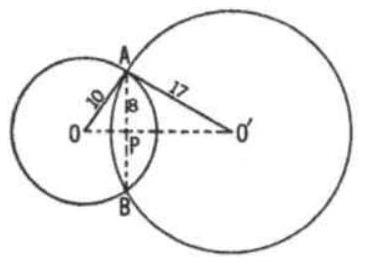
\includegraphics[width=\textwidth]{images/177(1).jpg}

The Pythagorean Theorem applied to right triangles \(O P A\) and \(O^{\prime} P A\) yields \(O P^{2}=O A^{2}-A P^{2}=10^{2}-8^{2}=36\),\\
\(O P=6\),


And \(O^{\prime} P^{2}=O^{\prime} A^{2}-A P^{2}=17^{2}-8^{2}=225, \quad O^{\prime} P=15\).\\
The distance between the centers of the circles is \(15+6=21\).


\end{document}
